\chapter{Extraktion raumakustischer Parameter}
\section{Die Nachhallzeit $\mathbf{RT_{60}}$}
\label{sec:rt60}
Als erstes entfernen wir den im Signal enthaltenen Teil vor dem eigentlichen Beginn der zu analysierenden Impulsantwort.
Als Kriterium zur Bestimmung des zeitlichen Nullpunkts der Impulsantwort verwenden die Position des ersten lokalen Maximums vor dem absoluten Maximum .
Zur Bestimmung der Nachhallzeit der gegebenen Impulsantwort haben wir die Schroeder Methode \cite{Schroeder65} verwendet.
Dafür haben wir in MatLab zunächst folgende, diskretisierte Version $R[n]$ der Gleichung berechnet:
\begin{align*}
R[n] = \sum_{i=1}^N h^2[i] + \sum_{i=1}^n h^2[i]
\end{align*}
Aus diesem Vektor lässt sich wiederum eine diskretisierte Form der Energy Decay Curve berechnen, welche den auf 0 dB normierten Pegelabfall des Signals  beschreibt:
\begin{align*}
EDC_{norm}[n] = 10 \mathrm{log} \left(\frac{R[n]}{\sum_{i=1}^N h^2[i]}\right)
\end{align*}
Um daraus nun einen Wert für die Nachhallzeit T$_60$ zu bestimmen, haben wir T$_{20}$ und T$_{30}$ berechnet.
Dabei haben wir zunächst Indexdifferenzen gebildet und diese dann in Zeitwerte umgerechnet.
Für T$_{20}$ haben wir die Punkte die Pegelabfällen zwischen -5 dB und -25 dB in $EDC_{norm}[n]$ entsprechen verwendet, für T$_{30}$, die Differenz zwischen den -5 dB und -35 dB Punkten.
Dieses Vorgehen entspricht der DIN Norm .......? .
  




\begin{figure}[H]
    \center
    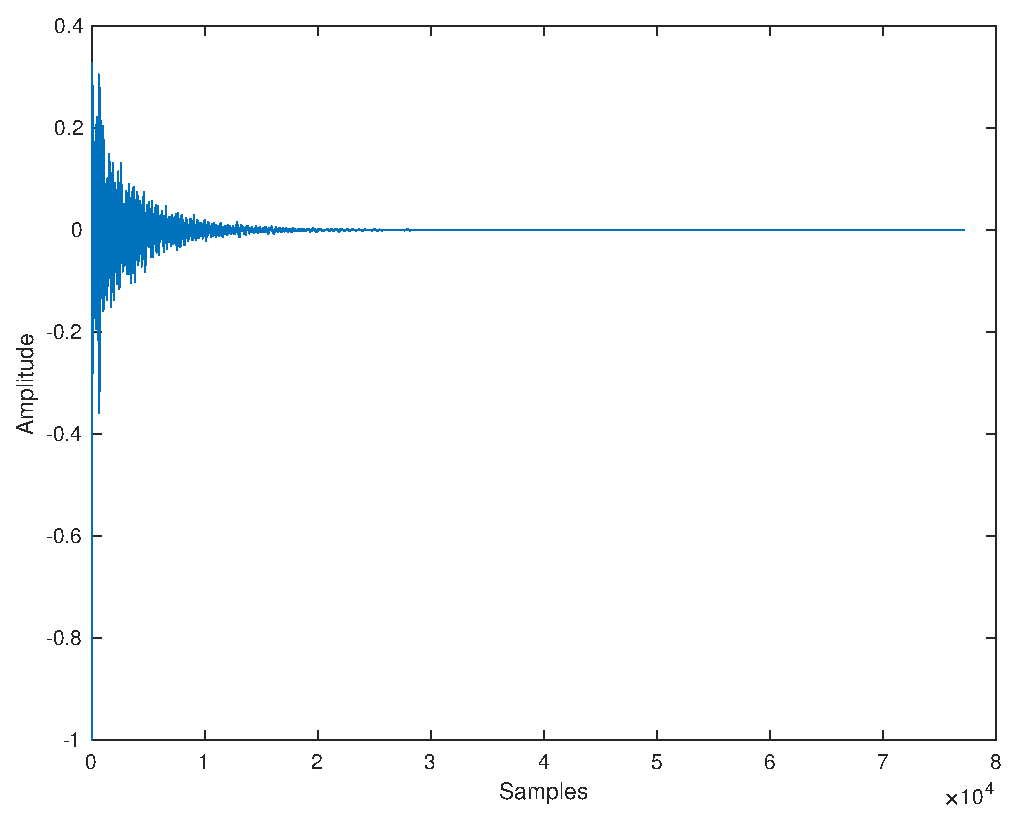
\includegraphics[width = 0.7\textwidth]{figures/samples}
    \caption{Die Impulsantwort}
    \label{fig:im}
\end{figure}

\begin{figure}[H]
    \center
    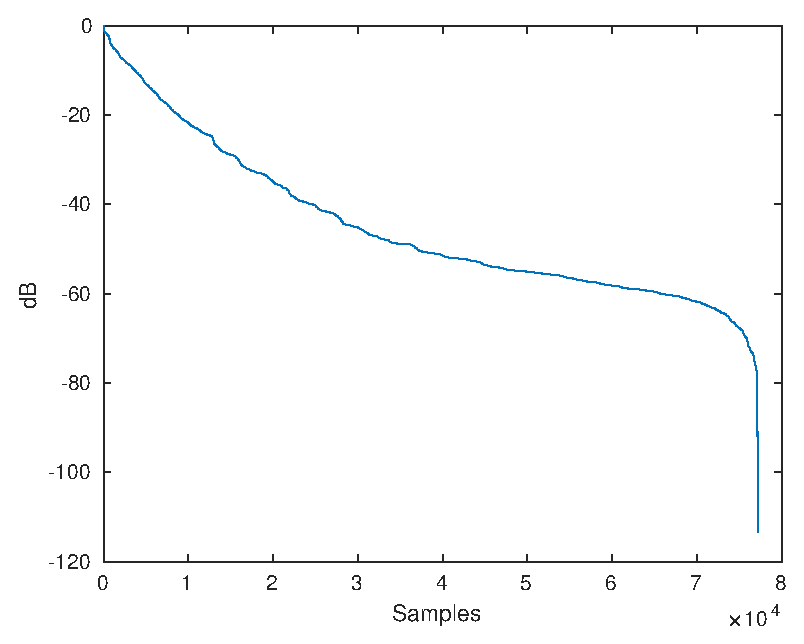
\includegraphics[width = 0.7\textwidth]{figures/EDC_norm.eps}
    \caption{EDC norm}
    \label{fig:edc}
\end{figure}

\section{Das Bassverhältnis $\mathbf{BR}$}
\label{sec:br}


\section{Das Klarheitsmaß $\mathbf{C_{80}}$}
\label{sec:c80}


\section{Der interaurale Kreuzkorrelationkoeffizient $\mathbf{IACC}$}
\label{sec:iacc}
Für den IACC wählen wir den

\begin{table}
    \centering
    \caption{Die Werte für $IACC_{Early}$ und $IACC_{Late}$}
    \label{tab:iacc}
    \begin{tabular}[\textwidth]{|l|l|l|}
        \hline
        Oktavbänder & Early & Late \\
        \hline
        125 & 0.9890 & 0.9355 \\
        \hline
        250 & 0.8986 & 0.7937 \\
        \hline
        500 & 0.2102 & 0.1034 \\
        \hline
        1000 & 0.4616 & 0.1902 \\
        \hline
    \end{tabular}
\end{table}

\section{Betrachtung der vier Oktavbänder}
\label{sec:bands}


\section{Vergleich der Nachhallzeiten}
\label{sec:ts}


\section{Die Schalldruckpegelverteilung}
\label{sec:sdpv}